  {\large \fontB Description:}
  
  {\bf solL} is a 2-dimensional analytical solution to the Cauchy equations with the acceleration term set to zero
  to represent creeping flow. The boundary conditions are free-slip everywhere on a unit domain. 
  This solution has an upper triangular block of density $\rho = \sigma_B$ above
      a lower block of density $\rho = \sigma_A$.
  \\

  {\large \fontB Parameters:}
 
  The variable parameters of this solution are:
  \begin{itemize}
    \item{density parameters: $ \sigma_B $ and $ \sigma_A $.}
    \item{viscosity: $\eta$ .}
    \end{itemize}

  \begin{SCfigure}[][h]
    \includegraphics[width=6cm,clip]{../figs/figL.eps}
    \caption[Short caption]{\label{figL} 
      Solution ({\bf SolL}):
      This solution has an upper triangular block of density $\rho = \sigma_B$ above
      a lower block of density $\rho = \sigma_A$.
      The boundary conditions are free slip everywhere on the surfaces of the unit box.}
  \end{SCfigure} 
  

